A tout moment, vous pouvez changer l’email de votre compte ChromaCase.
\\\\
Pour changer votre adresse email, rendez vous sur la page des réglages (Voir Capture \ref{fig:access-settings-mail}).

\begin{figure}[H]
	\begin{subfigure}[b]{0.7\textwidth}
		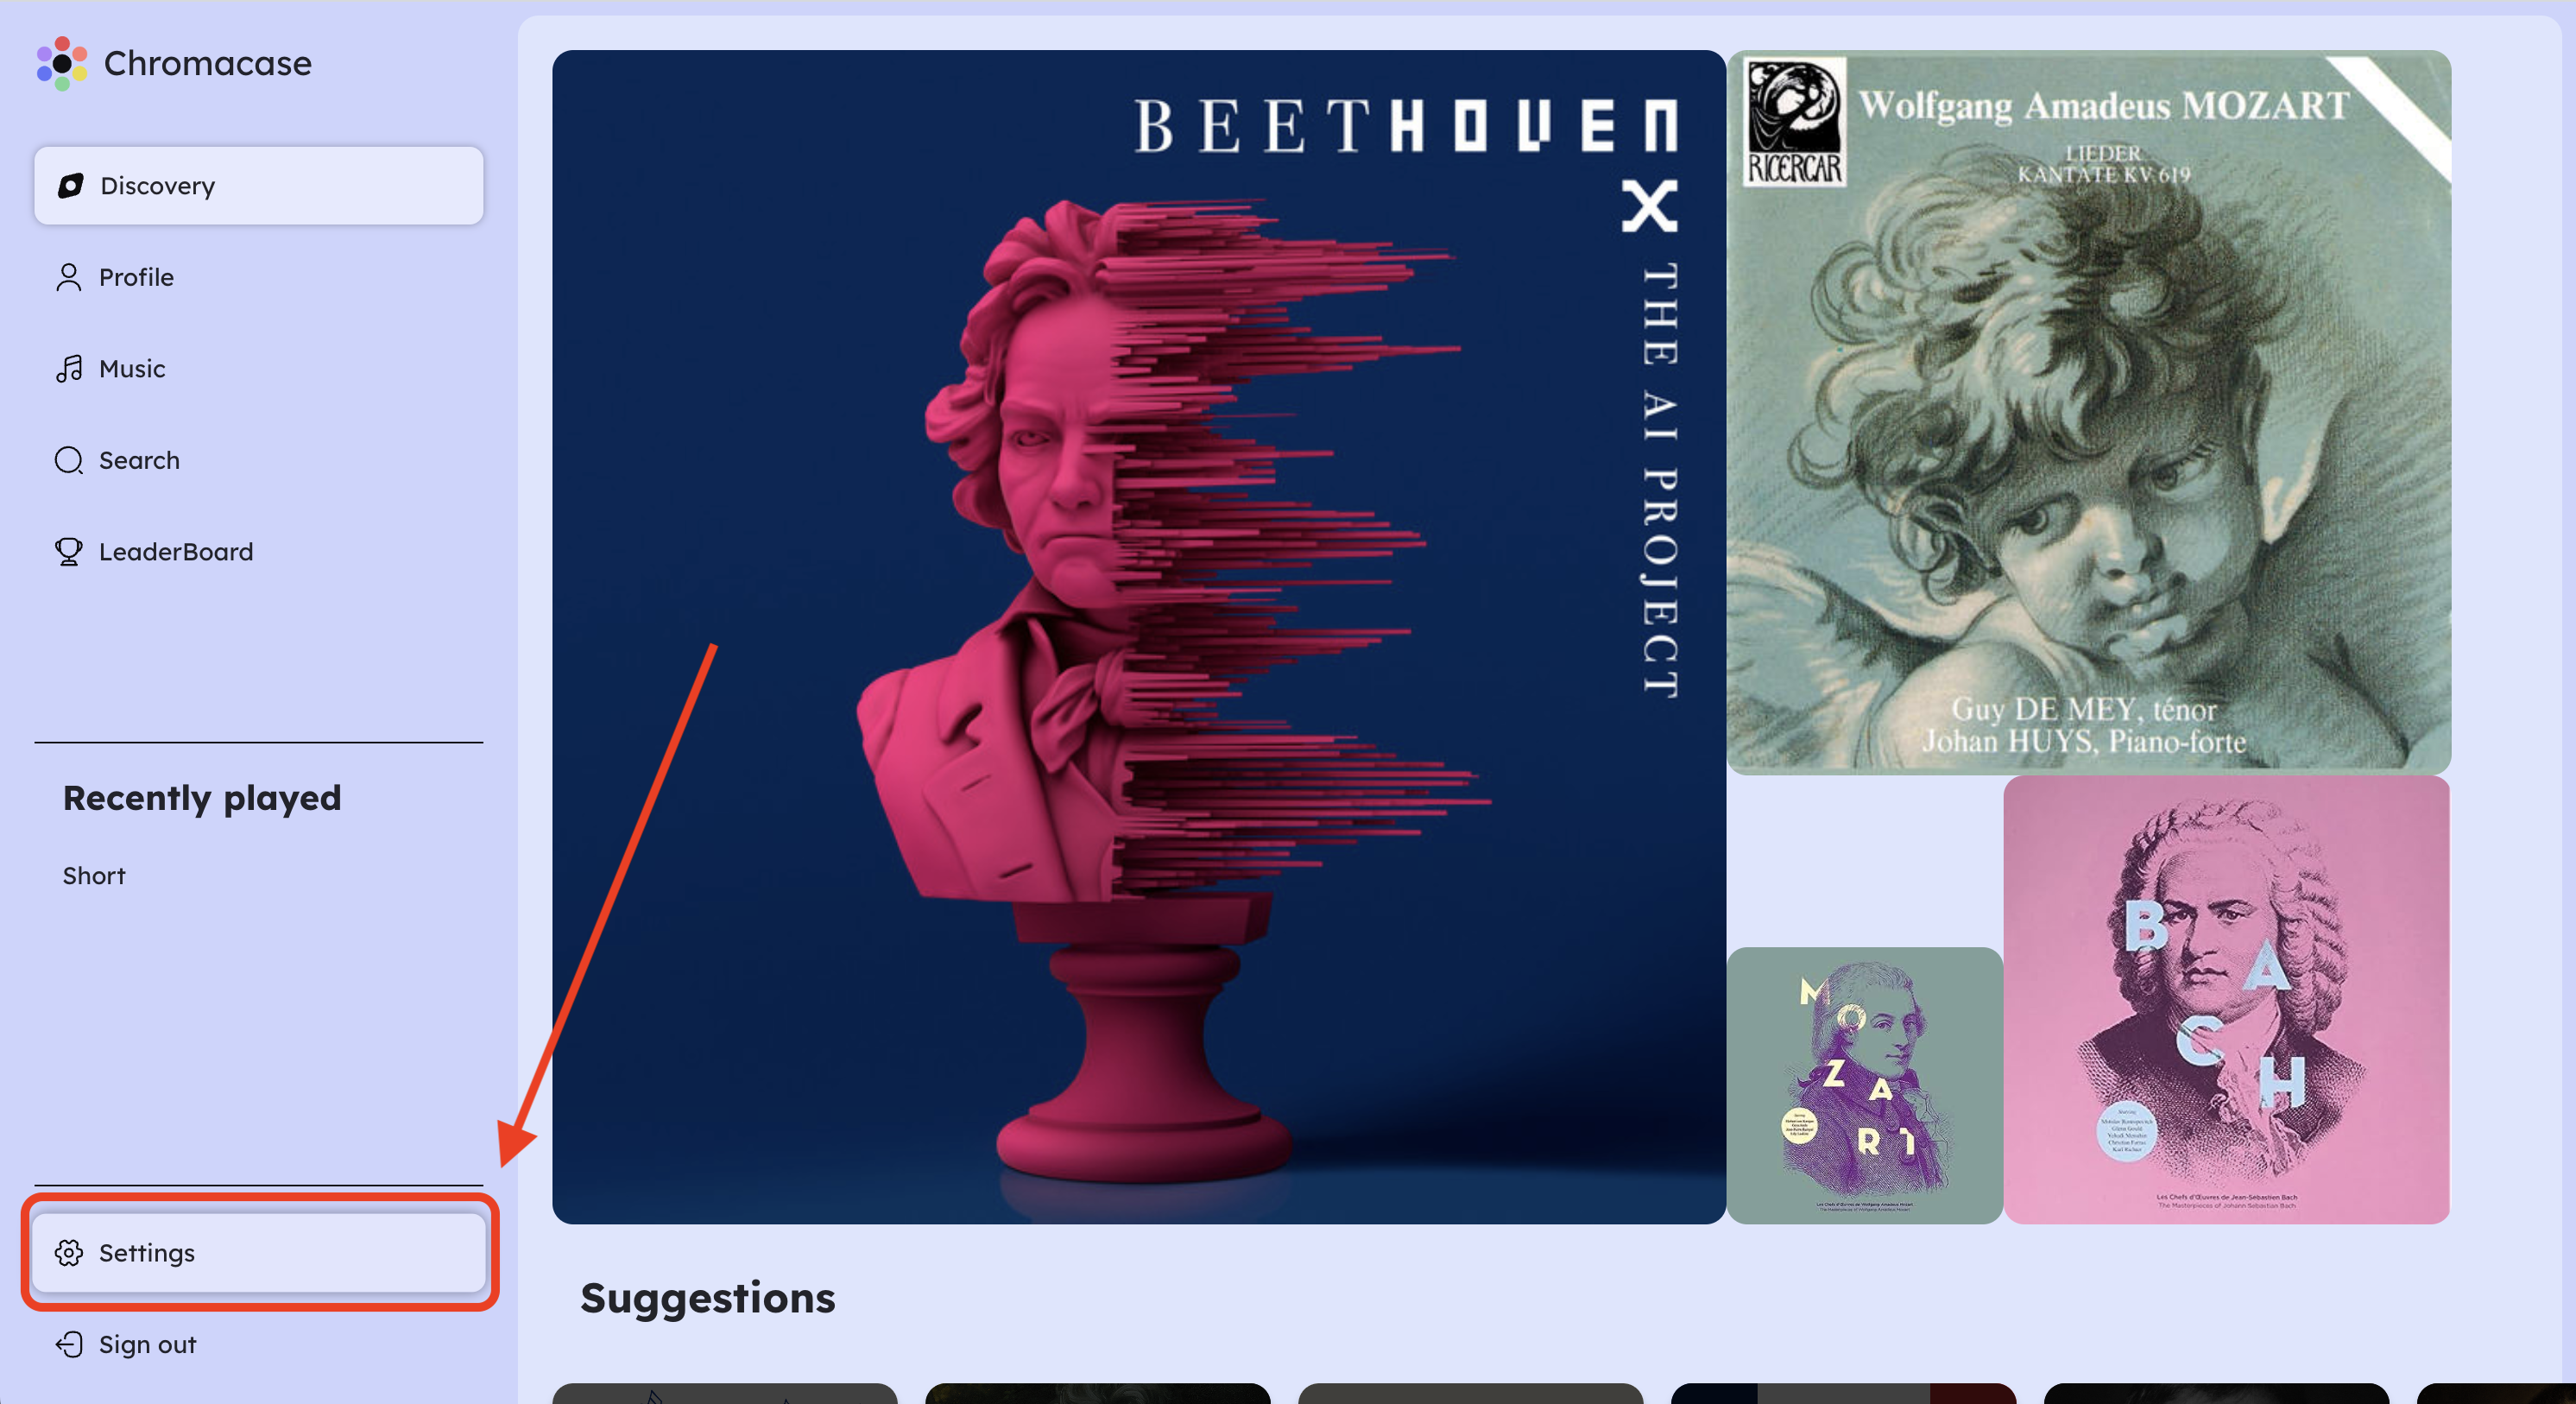
\includegraphics[width=\linewidth]{../\dir/guide/auth/access-settings.png}
		\caption{Version navigateur}
	\end{subfigure}
	\begin{subfigure}[b]{0.25\textwidth}
		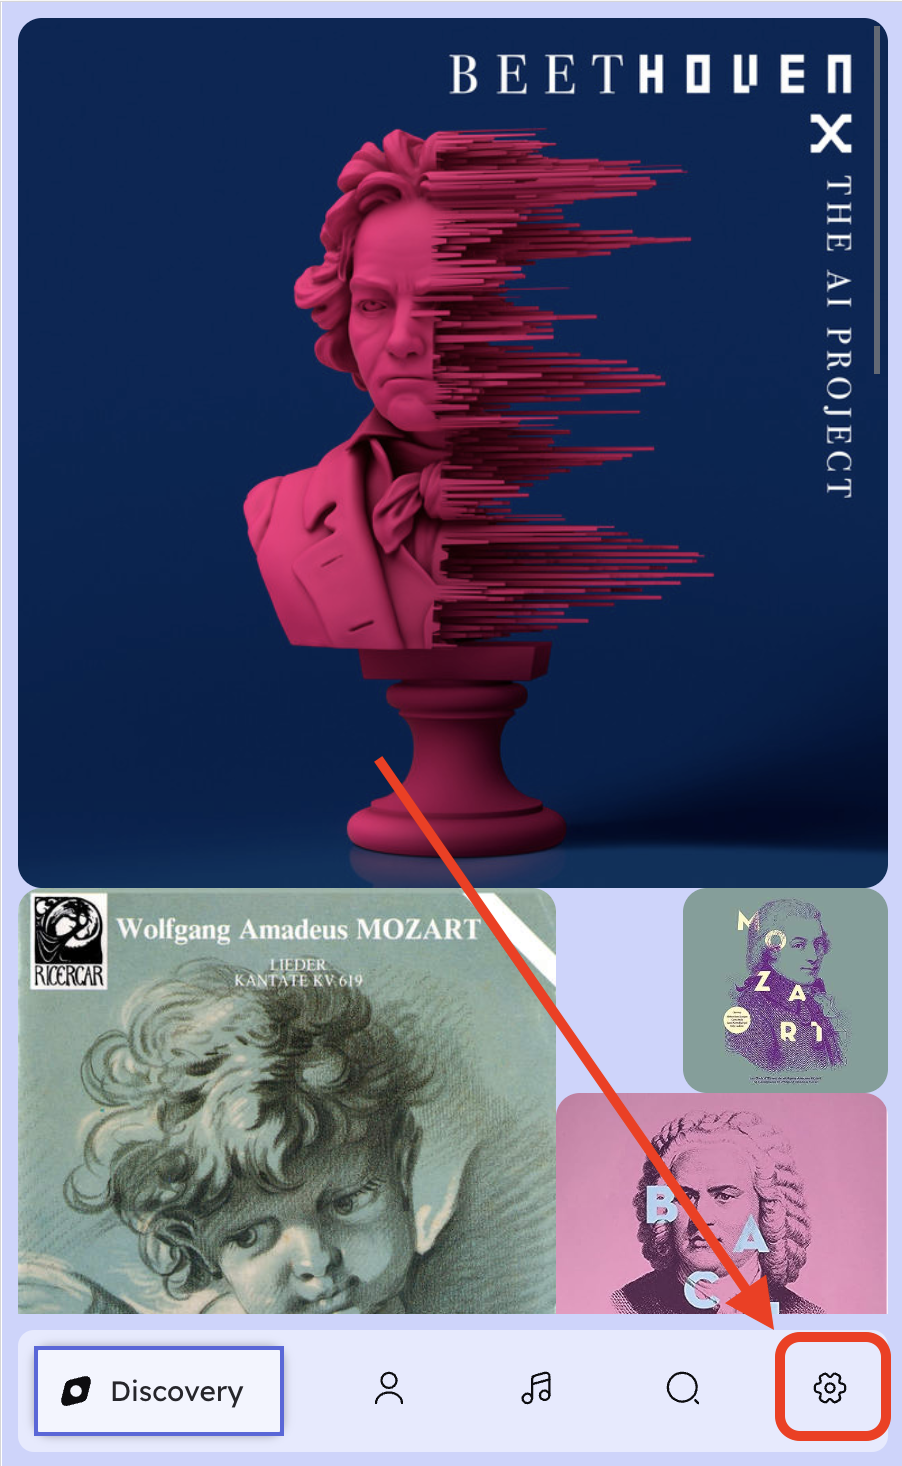
\includegraphics[width=\linewidth]{../\dir/guide/auth/access-settings-mobile.png}
		\caption{Version mobile}
	\end{subfigure}
	\caption{Accéder aux reglages}
	\label{fig:access-settings-mail}
\end{figure}

Cliquez sur l'onglet "Profile", puis "Changer l'Email", saisissez votre ancien et nouvel email dans les champs correspondants. Une fois le formulaire rempli, cliquez sur le bouton de validation (Voir Capture \ref{fig:change-mail}).

\begin{figure}[H]
	\begin{subfigure}[b]{0.7\textwidth}
		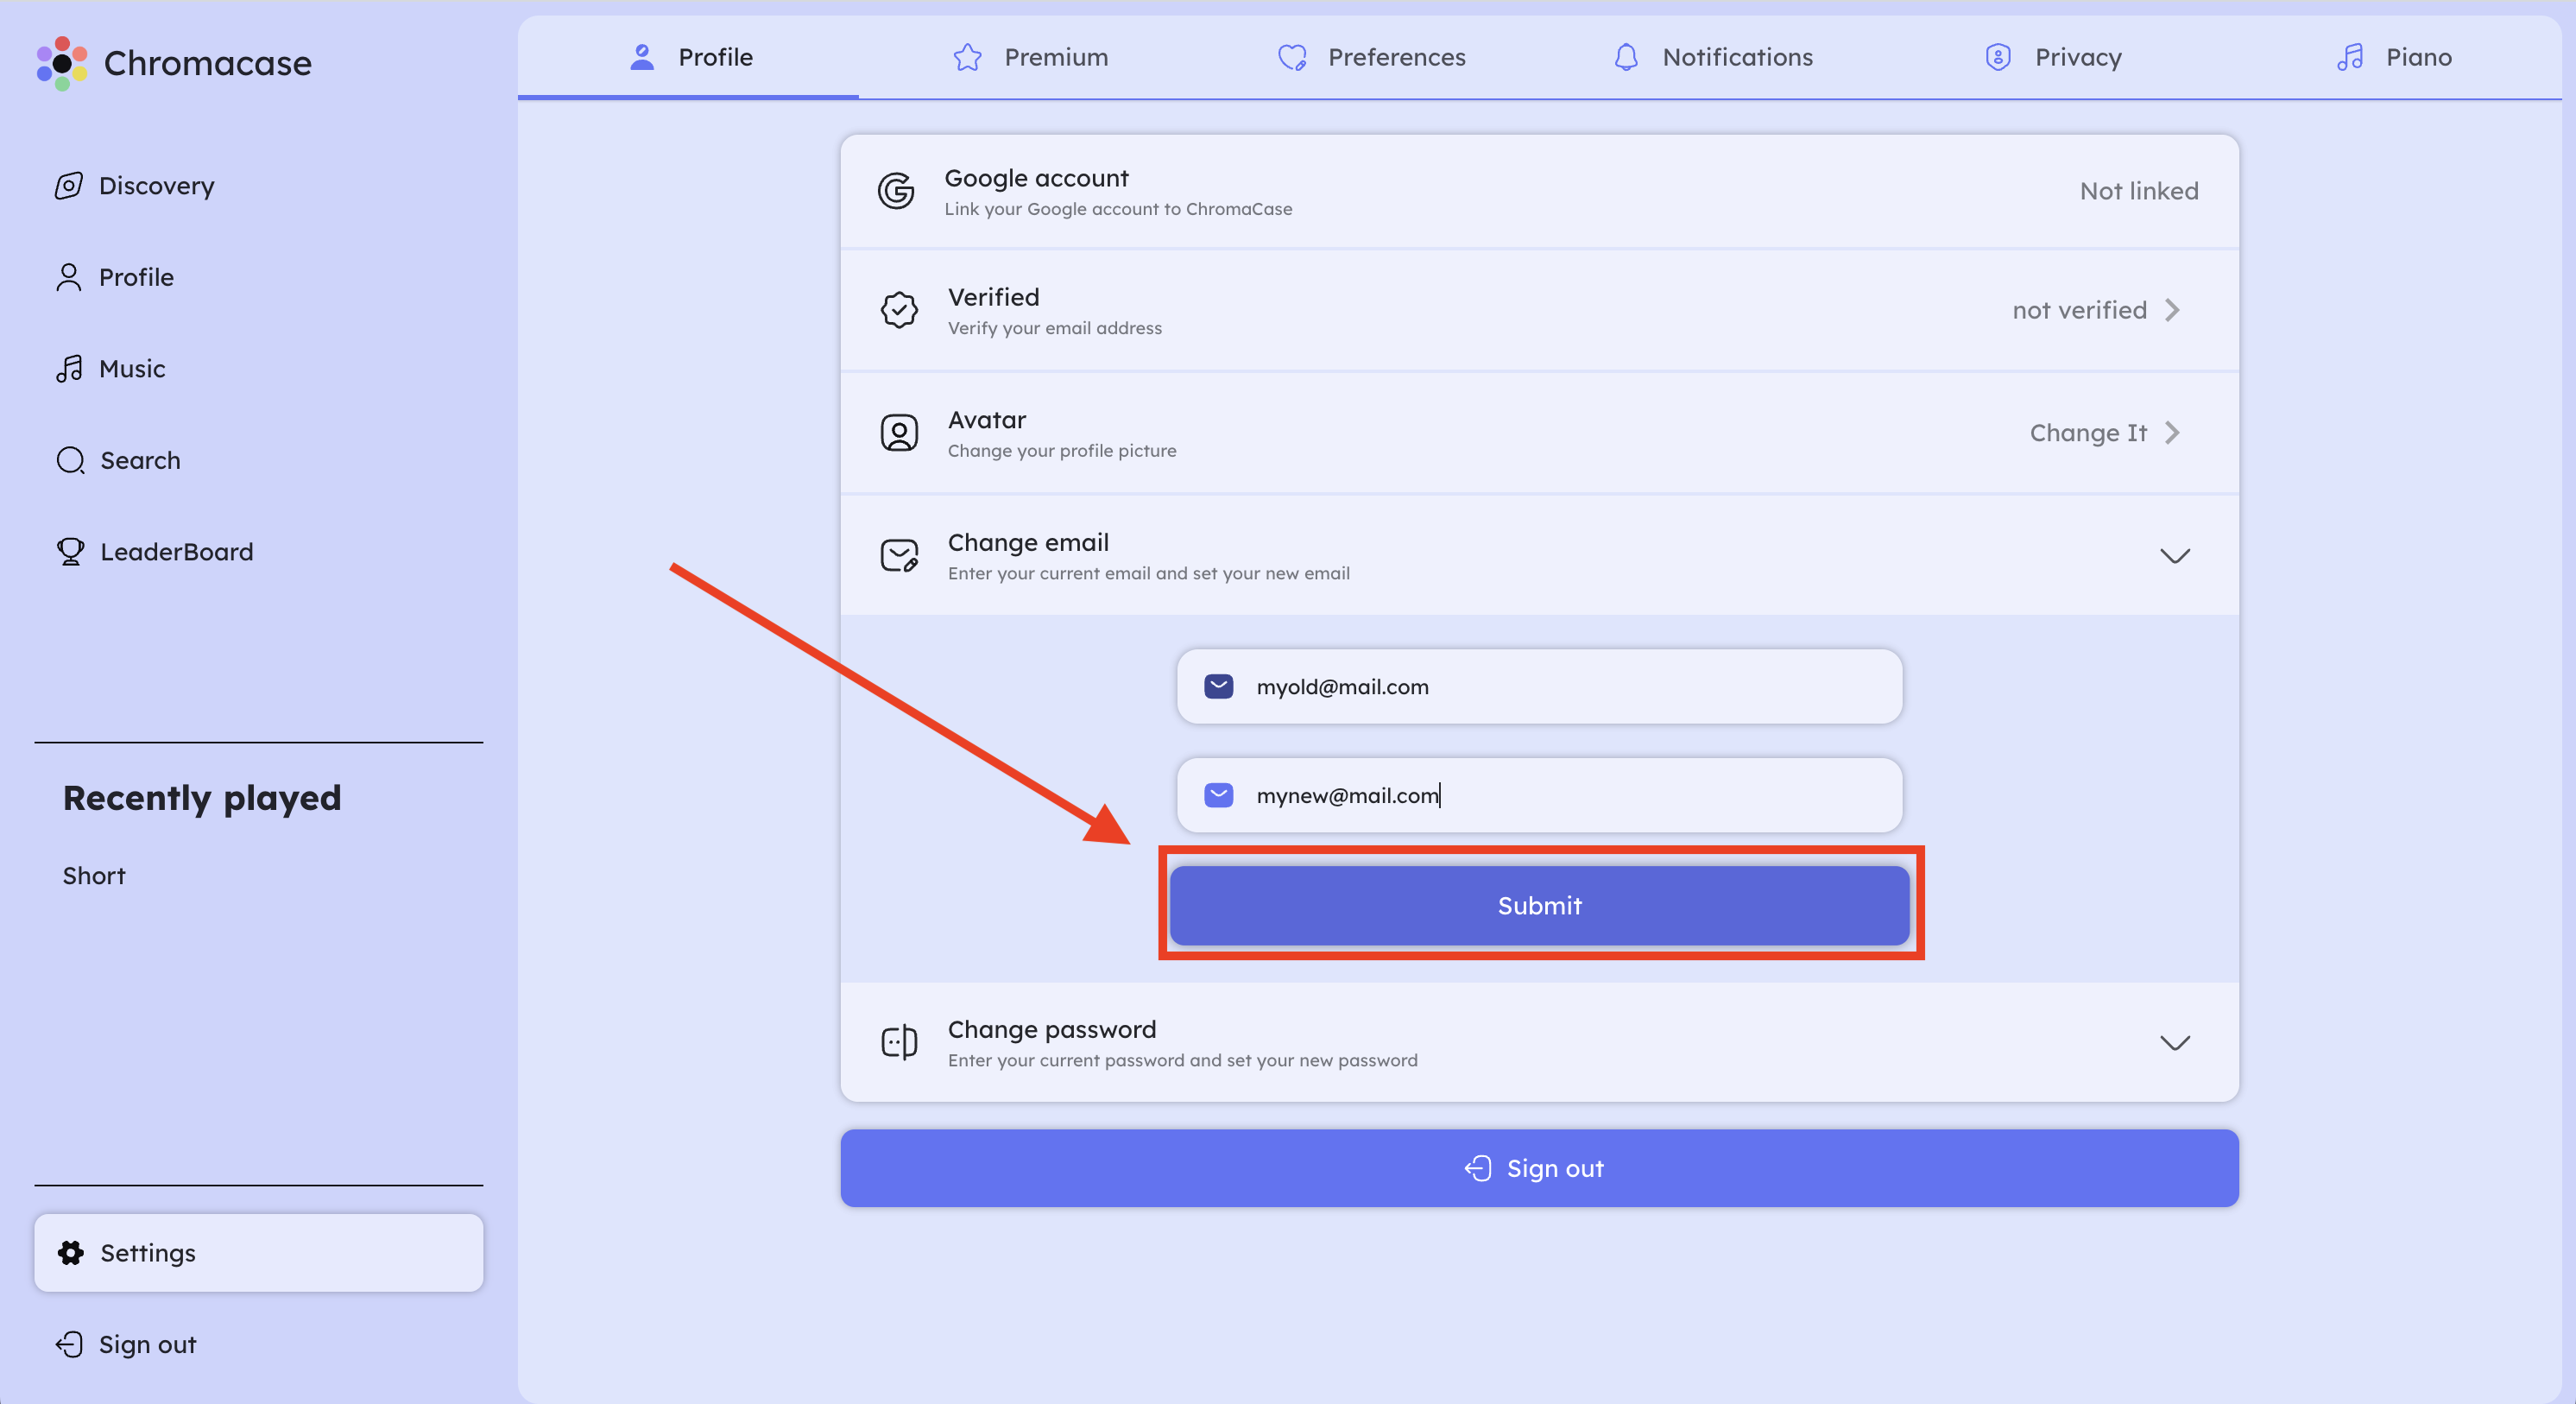
\includegraphics[width=\linewidth]{../\dir/guide/auth/change-mail.png}
		\caption{Version navigateur}
	\end{subfigure}
	\begin{subfigure}[b]{0.25\textwidth}
		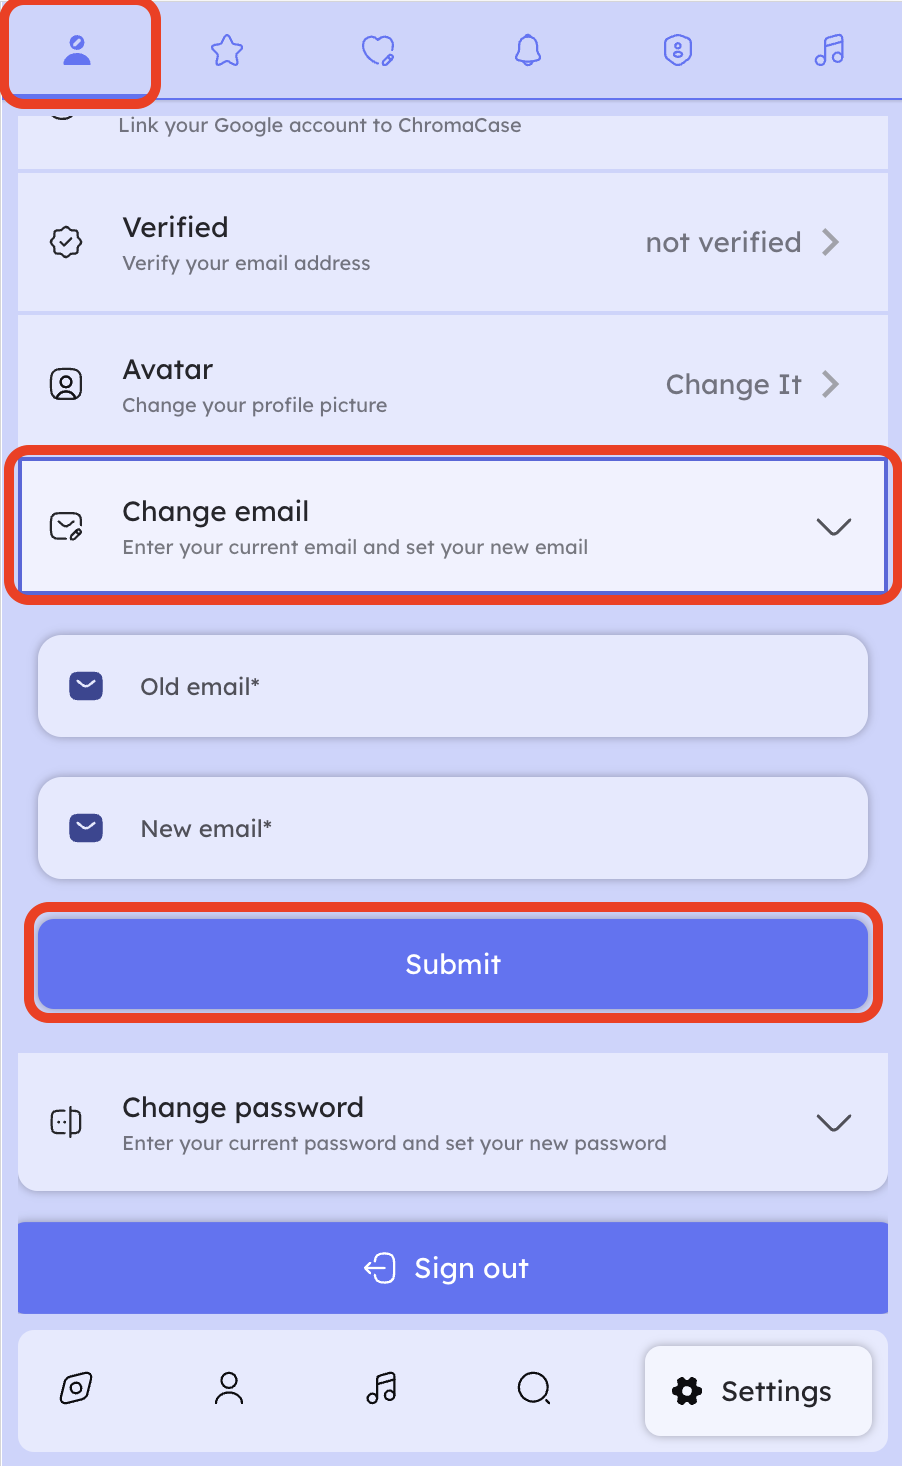
\includegraphics[width=\linewidth]{../\dir/guide/auth/change-mail-mobile.png}
		\caption{Version mobile}
	\end{subfigure}
	\caption{Changer d'email}
	\label{fig:change-mail}
\end{figure}